\documentclass[12pt]{book}

\usepackage[toc]{appendix} % para crear ambientes de apéndice
\usepackage{amsmath,amssymb, amsthm} % Para mejorar ecuaciones
\usepackage[utf8]{inputenc}
\usepackage[spanish]{babel} % Español
\usepackage[nice]{nicefrac}  % Para mejorar fracciones
\usepackage{graphicx} % Para insertar graficos
\usepackage{float} % Para manejar la ubicacion de graficos
\usepackage[colorlinks=true, allcolors=black]{hyperref} % Para hipervincular las referencias dentro del texto
\usepackage[Conny]{fncychap} % Capítulos

\usepackage{marginnote}% Paquete para notas al márgen
    \setlength{\marginparwidth}{4cm} % Ancho de la nota al margen
    \setlength{\marginparsep}{0.5cm} % Distancia mínima entre la nota y el texto principal
\usepackage{multirow,array}


\begin{document}

Borradores de los apuntes para el ramo de Economía Política con el profesor Óscar Landerretche. Podría contener errores y en caso de encontrarlos agradecería que me los hiciera notar al correo: joamartine@fen.uchile.cl

Última actualización: \today 

\newpage

\setcounter{chapter}{3}

\chapter{El Problema del tiempo y del riesgo}

\section{Optimización intertemporal y la aversión al cambio}
\subsection{Introducción al modelo de consumo intertemporal}
El economista y estadístico \textbf{Irving Fisher}\marginnote{\textbf{Irving Fisher 1867-1947:} Economista y estadístico estadounidense reconocido por sus avances en la teoría económica (Ecuación de Fisher, hipótesis de Fisher, teorema de separabilidad de Fisher...).} desarrolló en gran parte uno de los modelos más influyentes en como entendemos que se toman las decisiones de consumo a lo largo del tiempo. Para esto tenemos que pensar en un individuo que se detiene a pensar en el presente cuanto consumirá ahora y cuanto consumirá en cada período en el futuro. 

Este modelo considera un consumidor racional que enfrenta restricciones a su consumo a lo largo del tiempo. Una simplificación que haremos para presentar el modelo será que el consumidor solo vive dos períodos. 

Uno de los factores más importantes de este modelo es la capacidad de que el individuo ahorre y contraiga deuda. Es la manera en que el consumidor podrá transportar dinero del presente al futuro (ahorro) o viceversa del futuro al presente (deuda).

Partiremos armando intuitivamente la restricción de cada período para así juntarlas y obtener lo que llamaremos una \textbf{restricción intertemporal}.

\subsection{Restricción intertemporal}
\marginnote{\textbf{Restricción intertemporal:} Restricción resultante de consumir con un ingresos finitos transferibles entre períodos de tiempo}
El individuo representativo partirá consumiendo en el período uno ($c_1$), para financiar su consumo recibirá un ingreso $y_1$. Lo primero que podemos sacar es que el individuo va a estar restringido pues todo consumo debe estar respaldado por ingreso, $y_1 \geq c_1$. Aquí vamos a añadir otro factor a la mezcla, el individuo podrá ahorrar o endeudarse. Este factor ahorro/deuda lo denotaremos por $s$, será $>0$ cuando se trate de ahorro y será $<0$ cuando sea deuda.

Con esto ya podemos definir la restricción en el primer período como la ecuación \ref{eq: rest 1}.
\begin{equation}
    y_1 = c_1+s \label{eq: rest 1}
\end{equation}

En el segundo período la restricción seguirá la misma lógica, lo que hay que considerar adicionalmente es que hay una tasa de interés ($r$) de por medio para cuando uno ahorra o se endeuda. Por lo que los ingresos $y$ en un período, se convertirán en $y(1+r)$ en el siguiente período.

La restricción del segundo período puede ser descrita como la ecuación \ref{eq: rest 2}.
\begin{equation}
    y_2 = c_2 - s(1+r) \label{eq: rest 2}
\end{equation}

Teniendo las restricciones para los dos períodos podemos describir una restricción intertemporal combinandolas. Para esto reemplazamos $s$ de \ref{eq: rest 1} en \ref{eq: rest 2}.
\begin{equation*}
    y_2 = c_2 - (1+r)(y_1-c_1) 
\end{equation*}

Reordenando podemos encontrar dos expresiones útiles que representan la misma restricción, las dos significan que todo el consumo tiene que ser financiado por ingreso. 

La expresión \ref{eq: valor futuro} está ordenada de forma que los ingresos presentes sean traídos a \textbf{valor futuro},\marginnote{\textbf{Valor futuro:} El valor que tendrá cierta monto en un período futuro dadas las oportunidades de ahorro/inversión.}[-4cm]mientras que \ref{eq: valor presente} está expresado de forma en que los ingresos futuros sean traídos a \textbf{valor presente}.\marginnote{\textbf{Valor presente:} El valor que tiene cierto monto en el futuro traído a lo que valdría hoy dadas las oportunidades de ahorro/inversión.}
\begin{align}
    y_1(1+r) + y_2 &= c_1(1+r) + c_2 \label{eq: valor futuro} \\
    \quad & \quad \notag\\
    y_1 + \frac{y_2}{1+r} &= c_1 + \frac{y_2}{1+r} \label{eq: valor presente}
\end{align}

Esta restricción intertemporal puede ser graficada tal como una restricción presupuestaria (Véase la figura \ref{fig: restricción intertemporal}). De esta recta el consumidor decidirá en qué punto maximiza su utilidad, de este punto sabremos si el consumidor se está endeudando o ahorrando. 
\begin{figure}
    \centering
    \caption{Restricción intertemporal}
    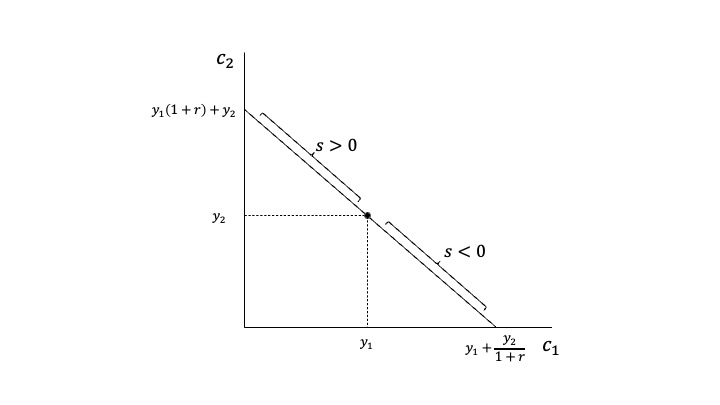
\includegraphics[width=\textwidth]{Figuras/CI Restriccion intertemporal.jpeg}
    \label{fig: restricción intertemporal}
\end{figure}

El punto en que el consumidor elija para maximizar su utilidad podrá ser utilizado para ver si está ahorrando o endeudándose. Es directo ver que si $c_1>y_1$ implica que $s<0$, es decir se está contrayendo deuda para financiar el consumo presente. Para financiar esa deuda el consumidor estará obligado en el futuro a que $c_2<y_2$ pues cierta parte va a ser usada para pagar la deuda. Tanto este caso como el caso en que el individuo ahorra se pueden ver en la figura \ref{fig: restricción intertemporal}.

Por otro lado es relevante entender por qué el consumo máximo de $c_2$ en la figura está en valor futuro, mientras que el consumo máximo $c_1$ está en valor presente. 

Un caso que se verá más adelante son las restricciones de liquidez, es decir cuando la tasa a la que uno se endeuda es más alta a la cual uno ahorra.\footnote{Un caso extremo en que la tasa a la que uno se endeuda tiene a infinito llevará inevitablemente a este consumidor racional a comportarse como un consumidor keynesiano.} 

\subsection{El consumidor}

El consumidor racional en esta ocasión maximizará utilidad mediante consumo en dos períodos. Tendrá una función de utilidad para un período $i$ tal que $u'(c_i)>0$ y $u''(c_2)<0$, es decir, es decir cada unidad de consumo tendrá efectos positivos sobre su utilidad pero a rendimientos decrecientes. La concavidad de la función de utilidad se puede interpretar como que el individuo es saciable y esa es una de las razones por las que preferirá suavizar su consumo a lo largo del tiempo

La utilidad entre estos dos períodos puede ser expresado simplemente como la suma entre $u(c_1)$ y $u(c_2)$ pero añadiremos un matiz más. El consumidor tendrá una preferencia por el consumo en el presente por sobre el consumo en futuro. Para modelar esta preferencia añadiremos una \textbf{tasa de impaciencia} que descontará el consumo en futuro. Podemos expresar la función de utilidad entre los dos períodos en la ecuación \ref{eq: ut intertemporal}.
\begin{equation}
    U(c_1,c_2) = u(c_1) + \frac{1}{1+\rho} u(c_2) \label{eq: ut intertemporal}
\end{equation}
Por conveniencia podemos hacer un cambio de variable y definir $\beta = \frac{1}{1+\rho}$. 

\subsection{El problema y resolución del consumidor}
Ahora podemos plantear el problema del consumidor como una función a maximizar sujeto a una restricción.
\begin{align*}
        \max_{c_1,c_2} & \quad \Bigl\{ u(c_1) + \beta u(c_2) \Bigr\} \\ s.a.& \quad  y_1 + \frac{y_2}{1+r} = c_1 + \frac{c_2}{1+r}
\end{align*}
Para resolver este problema definimos el lagrangeano y derivamos las condiciones de primer orden. 
\begin{align}
        \mathcal{L}:& u(c_1) + \beta u(c_2) + \lambda \left( y_1 + \frac{y_2}{1+r} - c_1 - \frac{c_2}{1+r} \right) \notag \\
        \text{CPO:} \quad & \frac{\partial \mathcal{L}}{\partial c_1} = u'(c_1) - \lambda = 0 \notag \\
        &\frac{\partial \mathcal{L}}{\partial c_2} = \beta u'(c_2) - \frac{\lambda}{1+r} = 0 \notag \\
        & \lambda = \lambda \longrightarrow u'(c_1) = \left( \frac{1}{1+\rho} \right) u'(c_2)(1+r) \notag \\
        &  \frac{u'(c_1)}{u'(c_2)} = \frac{1+r}{1+\rho} \label{eq: perfil del consumidor}
    \end{align}
El resultado de la optimización va a ser la expresión \ref{eq: perfil del consumidor}, conocida como la \textbf{ecuación de Euler del consumo}. Esta ecuación se puede interpretar como el perfil del consumidor, como se ajusta el consumo en cada período dada la tasa de interés y la tasa de impaciencia. 

Por ejemplo, un aumento de la tasa de interés tiene un efecto positivo sobre el consumo futuro en relación con el consumo presente. Que el consumo presente disminuya implica que la utilidad marginal del consumo presente aumente\footnote{Esto debido a los rendimientos decrecientes de la utilidad del consumo.} esto tendría el efecto contrario en el consumo futuro. 

\subsection{Tasa de interés y tasa de impaciencia}

Hasta ahora solo hemos mencionado estas tasas como factores que considera el consumidor para mover su dinero entre períodos. Lo primero que se busca entender es que son fuerzas contrarias, una lleva consumo del presente al futuro y la otra del futuro al presente. Una forma más formal de empezar a entender estas fuerzas es como precios relativos de cada consumo

El precio relativo de consumo presente en relación al consumo futuro es la tasa de interés, puesto que el dinero que no se gaste en el presente será $(1+r)$ más valioso en el futuro. En el perfil del consumidor \ref{eq: perfil del consumidor} un aumento de un $1\%$ en la tasa de interés tendrá un efecto de un $1\%$ en el consumo futuro en relación al consumo presente.

A continuación veremos un caso en que los cambios en los precios relativos del consumo en cada período no tienen una relación 1 a 1 con los ajustes. Es decir que la elasticidad entre estas variables no va a ser igual a 1.

\subsection{Funciones de utilidad con aversión al riesgo}

Un caso especial y muy utilizado para describir el consumo de agentes en la economía es el uso de funciones de utilidad que incluyan aversión al riesgo. Las funciones de aversión relativa al riesgo constante (CRRA) incluyen el factor aversión al riesgo como una variable $\sigma$ que tendrá un efecto sobre la magnitud de los ajustes ante cambios en las variables exógenas (Como la tasa de interés por ejemplo). 

Un función de utilidad CRRA se puede describir como la expresión \ref{eq: CRRA}.
\begin{equation}
    u(c)= \left\{ \begin{array}{lcc} \frac{c^{1-\sigma}-1}{1-\sigma} & \text{si} & \sigma >0,\sigma \neq 1 \\ \\ \ln{(c)} & \text{si} & \sigma = 1 \end{array} \right. \label{eq: CRRA}
\end{equation}

De la cual si resolvemos como hicimos en el consumo intermtemporal anterior llegaremos a una ecuación de Euler del consumo (expresada en \ref{eq: perfil con aversión al riesgo}). De aquí podemos definir la \textbf{elasticidad intertemporal de sustitución} como el cambio porcentual en la relación marginal de consumo 1 y 2 para un cambio del $1\%$ en el precio relativo del consumo en 1 (tasa de interés). 
\begin{equation}
    \left( \frac{u'(c_1)}{u'(c_2)} \right) ^\sigma=  \frac{1+r}{1+\rho}  \label{eq: perfil con aversión al riesgo}
\end{equation}

La elasticidad intertemporal de sustitución describe la magnitud en que el consumo presente y futuro se ajustan ante un cambio en las condiciones (tasa de interés e impaciencia). 
\begin{equation}
    \text{EIS} = - \frac{\partial \ln (u'(c_1)/u'(c_2))}{\partial \ln (1+r)} = \frac{1}{\sigma}
\end{equation}

Mientras mayor sea la aversión al riesgo ($\sigma$) el consumidor responderá en menor medida a cambios en estas variables. Es decir, un aumento de $1\%$ en el precio relativo del consumo presente en relación al consumo futuro tendrá un efecto $1/\sigma$ en la relación de consumo futuro y consumo presente.

Mientras mayor sea la $\sigma$ mayor será la aversión al riesgo, representado por una curva más cóncava. 

\subsection{Restricciones de liquidez}

Hasta ahora se ha asumido que la tasa a la que un individuo ahorra ($r$) y se endeuda ($r^*$) es la misma. Un acercamiento más realista es que la tasa que paga un deudor es mayor a la tasa que consigue alguien por ahorrar. 

Cuando hablamos de \textbf{restricciones de liquidez} específicamente nos referimos a restricciones al endeudamiento. Este margen puede deberse a que la tasa de endeudamiento considera un premio por riesgo cuando hay probabilidad de impago. Mercados financieros menos robustos, los cuales suelen estar presentes en países menos desarrollados suelen estar sujetos a mayores restricciones de liquidez, lo cual deriva en muchas implicancias macro y microeconómicas.\footnote{Efectos sobre inversión y aplificación del ciclo económico, racionamiento del crédito, ineficiencias que llevan a perpetuar la desigualdad, etc\ldots}

\begin{figure}[t]
    \centering
    \caption{Restricciones de liquidez y perdida de bienestar ahorradores y deudores}
    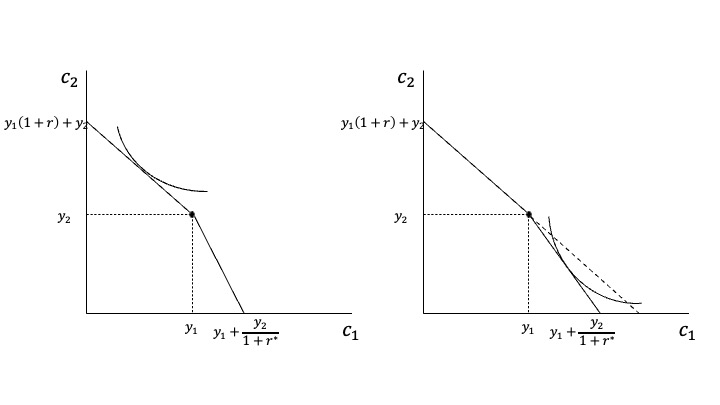
\includegraphics[width=\textwidth]{Figuras/CI Restricciones de liquidez.jpeg}
    \label{fig: Restricciones liquidez bienestar}
\end{figure}

Podemos ver los efectos en el bienestar de un consumidor bajo restricciones de liquidez en dos casos. Uno en el cual el consumidor prefiere ahorrar, en este caso se dice que la restricción no está activa puesto que las restricciones de liquidez solo afectan a la tasa de endeudamiento (Figura \ref{fig: Restricciones liquidez bienestar}). El caso en que el individuo preferiría endeudarse, en estas condiciones la restricción está activa, el punto que maximizaba el bienestar ya no es factible y por tanto hay una perdida en cuanto a utilidad. 

Es fácil ver que las restricciones tienen efectos negativos (o nulos) en el bienestar de las personas pues reduce la cantidad de opciones factibles en las que maximizar utilidad. 

\newpage

\section{Teoría de los mercados eficientes}
% explicación muy densa, revisitar y rescribir
Las finanzas, en parte, son una herramienta para enfrentarse a la incertidumbre. Al igual como puede ser el ahorro o un seguro las carteras de activos buscan minimizar el riesgo que enfrenta un inversor al buscar cierto retorno esperado. 

En 1952 \textbf{Harry Markowitz}\marginnote{\textbf{Harry Markowitz (1927-2023):} Economista estadounidense, premio nobel del 1990 gracias su aporte a la economía financiera.} presentó un modelo de formación de carteras en el cual inversores racionales con información respecto a los activos en disposición formarían una cartera riesgo-eficiente que se ajuste a sus preferencias de aversión al riesgo. El modelo de Markowitz no es tan complejo y maneja conceptos ya bastante discutidos en capítulos anteriores, como pueden ser individuos aversos al riesgo, maximizadores de utilidad sujetos a restricciones.

Anteriormente graficabamos la función de utilidad de un individuo como una función cóncava en caso de que este sea averso al riesgo. Una extensión del análisis sería armar curvas de diferencia entre el retorno esperado de un proyecto y el riesgo que conllevaría tomarlo. Esto es, para determinado rendimiento cuánto riesgo está determinado asumir el inversor. 
% Falta hacer un gráfico comparando las curvas de indiferencia de aversos, neutros y amantes del riesgo
\begin{figure}[ht]
    \centering
    \caption{Curvas de indiferencia riesgo-retorno}
    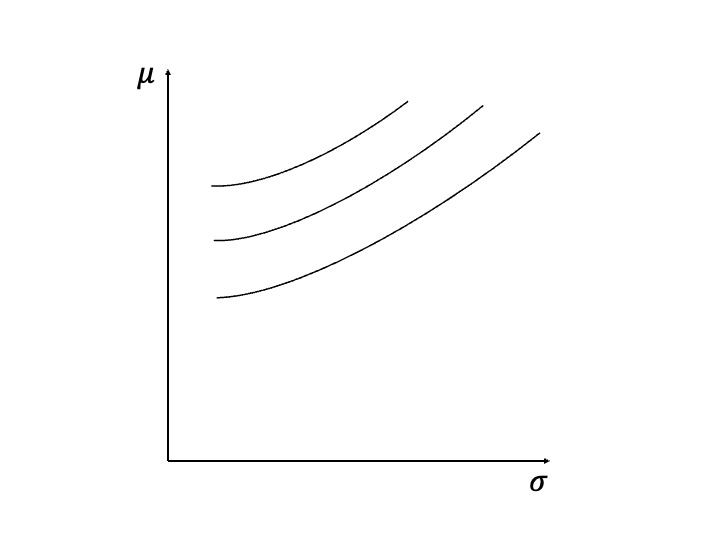
\includegraphics[width=10cm]{Figuras/Curvas de indiferencia riesgo-retorno.jpeg}
    \label{fig: Curvas de indiferencia riesgo-retorno}
\end{figure}
Los individuos preferirán un proyecto más riesgoso que otro siempre y cuando el rendimiento esperado sea suficiente o más para compensar la incertidumbre adicional. Las curvas de indiferencia (Figura \ref{fig: Curvas de indiferencia riesgo-retorno}) serán siempre convexas para todo individuo independiente si son aversos, neutros o amantes del riesgo. Sin embargo, mientras más aversos al riesgo sean más convexa será esta curva de indiferencia, dejándose ver que ante un mayor riesgo necesitan un incremento cada vez mayor de rendimiento esperado.

\subsection{Teoría de carteras, el problema financiero}

El problema de administración de \textbf{carteras}\marginnote{\textbf{Cartera de activos:} Una cartera o portafolio de activos hace referencia a una colección de distintos activos que se juntan en pos de diversificar riesgo.} hace referencia a la distribución y minimización del riesgo al buscar cierto retorno esperado. Las carteras son colecciones de activos los cuales tienen sus respectivos retornos y riesgos, cada activo puede estar más o menos presente en la cartera dependiendo de la composición de esta. 

El \textbf{precio} de una cartera en $t = 0$ puede ser descrito como la sumatoria del valor de los activos $A_i$ en dicho período.
\begin{equation}
    P_0 = \sum ^{I}_{i = 1} A_{i0}
\end{equation}
Mientras que el \textbf{retorno esperado}\marginnote{\textbf{Retorno esperado:} El retorno promedio de un activo o cartera de activos sujeto a incertidumbre y varianza.} que obtengamos de una cartera dependerá obviamente del retorno de cada activo, pero además del peso de dicho activo en la cartera. 
\begin{equation}
    r_p = \sum^{I}_{i = 1}\frac{A_{i0}}{P_0} r_{i0}
\end{equation}
Por otro lado, el riesgo\footnote{Con riesgo generalmente nos referimos a la desviación estándar del activo o portafolio.} de una cartera no se corresponde a simplemente la suma de las varianzas, esto ya que entra en juego las correlaciones de los activos entre sí. Es decir, no nos fijamos en como se comportan los activos por separado sino la combinación de dichos activos en un mismo portafolio. Veamos esto más en detalle:

Ahora mismo vamos a dejar de lado el tema riesgo-retorno para centrarnos en la minimización de riesgo, definiendo los puntos importantes que permiten que al juntar activos reduzcamos el riesgo del portafolio. Es necesario conocimientos elementales de estadística, los cuales se pueden encontrar en el anexo.

Para un portafolio de dos activos riesgosos $i$ con esperanza $\mu_i$ y varianza $\sigma^2_i$,
\begin{align*}
    X \sim (\mu_X,\sigma_X^2), \quad Y \sim(\mu_Y,\sigma_Y^2)
\end{align*}
El portafolio está compuesto por una fracción $0\leq a \leq 1$ de $X$ y por una fracción $0\leq b \leq 1$ de $Y$. Entonces podemos escribir la varianza del portafolio como $\mathbb{V}(aX + bY)$. Es decir, la suma de la varianza de los activos $X$ e $Y$ y de la covarianza entre los mismos. 
\begin{equation}
    \mathbb{V}(aX+bY) = a^2\sigma_X^2 + b^2\sigma_Y^2 + 2ab\text{Cov}_{XY} \label{eq: riesgo de portafolio suma}
\end{equation}
Como se puede observar la varianza del portafolio completo no es sólo la suma de las varianzas de los activos por separado sino también la interacción (covarianza) entre los mismos.

Es directo observar en \ref{eq: riesgo de portafolio suma} que si la covarianza entre los activos es positiva la varianza del portafolio será mayor que la suma de las varianzas. En este caso, se juntaron dos activos volátiles que juntos hacen una cartera aún más volátil, lo cúal a menos que presente rendimiento esperado tan alto que compense la incertidumbre, no valdría la pena. 

La idea del portafolio que estamos buscando en este momento es que reduzcamos el riesgo al que el inversor se enfrenta. Para esto se necesitan activos que juntos reduzcan el riesgo de portafolio, condición para esto es que sean independientes o que covarien negativamente. Obviamente si la covarianza en \ref{eq: riesgo de portafolio suma} es negativa el riesgo del portafolio bajará puesto que en caso de que a un activo le vaya mal lo más probable es que el otro la vaya bien.

Mostremos que aun cuando los activos son independientes el riesgo del portafolio baja. En caso de que $X$ e $Y$ fueran independientes implicaría que $\text{Cov}_{XY}= 0$. Asumiendo que tienen varianzas $\sigma_X^2 = \sigma^2_Y = 1$. Tendríamos que la desviación estándar del portafolio sería $\mathbb{SD}(aX + bY) = \sqrt{a^2 + b^2}$, mientras que la sumatoria de las desviaciones de los activos por separado serían $a+b$. Como se puede ver en la figura \ref{fig: Diversificación del riesgo con dos activos} por teorema de Pitágoras, siempre se cumplirá que $\sqrt{a^2 + b^2} < a+b$.

\begin{figure}[ht]
    \centering
    \caption{El riesgo de un portafolio será menor que la suma de los riesgos de los activos que lo componen}
    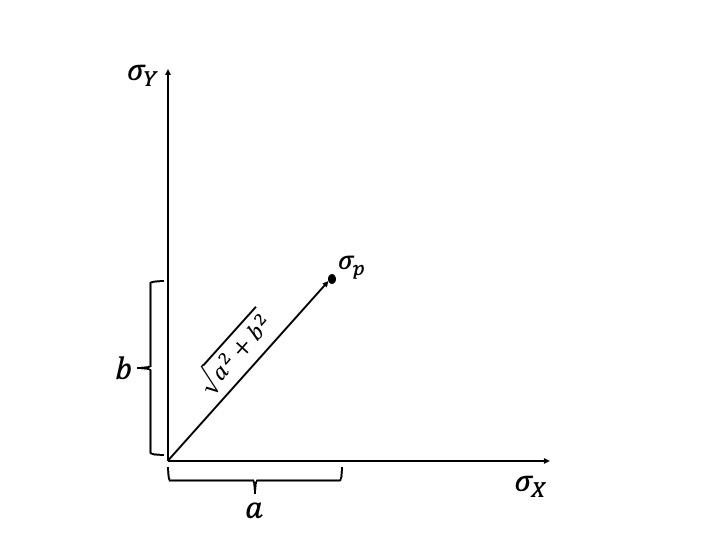
\includegraphics[width=11cm]{Figuras/Riesgo de un portafolio y reduccion de riesgo.jpeg}
    \label{fig: Diversificación del riesgo con dos activos}
\end{figure}

Reduciremos riesgo juntando activos siempre y cuando sean independientes o covaríen negativamente. En el caso anterior fueron dos activos, pero generalizemos para $N$. Formando una cartera de $N$ activos $X_i$ de igual varianza con pesos iguales cada uno, podemos escribir la varianza de la cartera de esta manera,
\begin{align*}
    \mathbb{V} \left(\sum_{i =1}^{N} \frac{X_i}{N} \right) = \frac{1}{N^2}\mathbb{V} \left(\sum_{i = 1}^N X_i \right) = \frac{N\sigma^2}{N^2} = \frac{\sigma^2 X}{N}
\end{align*}
Mientras más activos independientes conformen la cartera en partes iguales se diversifica el riesgo por lo que disminuye la varianza de la cartera.
\begin{equation}
    \lim_{N \to \infty} \frac{\sigma^2 X}{N} = 0
\end{equation}
Ahora finalmente definamos finalmente la varianza de una cartera de activos $i$ donde cada uno pesa una fracción $w_i$ en la cartera y tienen una varianza $\sigma^2_i$. 
\begin{equation}
    \sigma_{P_0}^2 = \sum_{i = 1}^I w_{i0}^2\sigma_i^2 + \sum^I_{i = 1}\sum^I_{i \neq j} w_{i0}w_{j0}\text{Cov}_{ij}
\end{equation}
Se lee como la sumatoría de las varianzas y sus respectivas ponderaciones más las covarianzas de todos los activos entre sí.

Al empezar a hablar de riesgo de portafolio dejamos de lado el análisis riesgo-retorno relacionado a las curvas de indiferencia. Ahora buscaremos relacionar la selección de cartera con las preferencias del inversor y sus curvas de indiferencia.

\newpage

\begin{appendices}
    \chapter{Apéndice}

\section{Random Walk}

Incluyendo incertidumbre a un modelo con expectativas racionales podemos obtener distintos resultados dependiendo del tipo de función de utilidad. En este caso veremos como un individuo neutro al riesgo sigue una trayectoria de consumo tipo \textit{random walk}.

Primero resolvamos el problema con un consumo futuro incierto.
\begin{align*}
    \max _{c_t , c_{t+1}} \quad  u(c_t)+ \mathbb{E}_t \{u(c_{t+1})\} \\ 
    s.a \quad y_t + \frac{y_{t+1}}{1+r} = c_t +\frac{c_{t+1}}{1+r}
\end{align*}

Planteamos el lagrangeano:
\begin{equation*}
    \mathcal{L}: u(c_t)+ \mathbb{E}_t \{ u(c_{t+1}) \} + \lambda \left(y_t + \frac{y_{t+1}}{1+r} - c_t - \frac{c_{t+1}}{1+r} \right)
\end{equation*}

Derivamos las condiciones de primer orden para encontrar la ecuación de Euler del consumo. 
\begin{align}
    \frac{\partial \mathcal{L}}{\partial c_t} =u'(c_t) -\lambda = 0    \notag \\   u'(c_t) = \lambda \\
    \frac{\partial \mathcal{L} }{\partial c_{t+1}} = \frac{1}{1+\rho} \mathbb{E}_t \{ u'(c_{t+1})\} - \frac{\lambda }{1+r} = 0 \notag 
 \\ \frac{1+r}{1+\rho } \mathbb{E}_t \{u'(c_{t+1})\} = \lambda \\
 u'(c_t) = \frac{1+r}{1+\rho} \mathbb{E}_t\{u'(c_{t+1})\} \label{eq: Ecuación de euler random}
\end{align}

La expresión \ref{eq: Ecuación de euler random} es la ecuación de Euler.

Para probar que un individuo neutral al riesgo sigue un \textit{random walk} en este caso podemos reemplazar la función de utilidad con una función cuadrática como en la expresión \ref{eq: ecuación cuadrática}. La utilidad marginal por tanto va a ser lineal lo cual describe un individuo neutro al riesgo.
\begin{equation}
    u(c_t) = bc_t - \frac{a}{2}c_t ^2 \label{eq: ecuación cuadrática}
\end{equation}

Remplazmaos las funciones de utilidad marginales en la ecuación de Euler del consumo y asumimos que $r=\rho = 0$:
\begin{align*}
    b-ac_t = \mathbb{E}_t\{b-ac_{t+1}\}
\end{align*}

Aplicamos propiedades de la esperanza y simplificamos los $b$ y $-a$:
\begin{equation}
    c_t = \mathbb{E}_t \{c_{t+1} \} \label{eq: random walk resultado}
\end{equation}
Según muestra la ecuación \ref{eq: random walk resultado} el consumo en $t$ va a ser igual a lo que se espera que sea el consumo en $t+1$. Por lo que la trayectoria de consumo se mantendrá igual hasta que llegue un shock que la desvíe.

\section{Incertidumbre y ahorro por precaución}

Bajo el mismo caso de incertidumbre, un individuo con aversión al riesgo tendrá un ahorro por precaución. Esto ya que no se cumple el caso de \ref{eq: random walk resultado} ya que tendremos utilidades marginales crecientes a tasas decrecientes. 

Esto se traduce en que la esperanza de la utilidad es mayor a utilidad de la esperanza
\begin{equation}
    \mathbb{E}_t \{ u(c_t) \} < u(\mathbb{E}_t \{ c_t \})
\end{equation}
Podemos derivar la expresión. 
\begin{equation}
    \mathbb{E}_t \{ u'(c_t) \} > u'(\mathbb{E}_t \{ c_t \})
\end{equation}
Según \ref{eq: Ecuación de euler random} (con $\rho = r = 0$) podemos reemplazar.
\begin{align}
    u'(c_t) = u'(\mathbb{E}_t \{ c_{t+1} \}) < \mathbb{E}_t\{ u'(c_{t+1}) \} \notag \\
    u'(c_t) < \mathbb{E}_t\{ u'(c_{t+1}) \} \label{eq: incertidumbre marginla averso}
\end{align}
De \ref{eq: incertidumbre marginla averso} podemos interpretar que debido al perfil del consumidor se consume menos por una necesidad de ahorro por precaución.

\section{Modelo CAPM de consumo}
Los retornos están sujetos a varianza. retornos puedes estar sujetos a varianza (incertidumbre). Para individuos con expectativas racionales que tienen la opción de consumir en el presente o de invertir para llevar dinero al futuro podremos llegar a la ecuación de euler del tipo \ref{eq: Ecuación de euler random}. Específicamente,
\begin{equation}
    u'(c_1) = \mathbb{E}_1  \left[  \frac{1+r^i}{1+\rho} u'(c_2)  \right] \label{eq: Ecuación de euler random 2}
\end{equation}
Donde $r^i$ es un activo con riesgo. Queremos buscar el diferencial entre la esperanza del activo riesgoso y el libre de riesgo. Utilizando las propiedades de la esperanza podemos desarrollar sacando el descuento intertemporal de la esperanza y multiplicando la esperanza de los retornos $1+r^i$ y $u'(c_2)$. Recordamos como desarrollar $\mathbb{E}(X\cdot Y)$ y aplicamos a \ref{eq: Ecuación de euler random 2}
\begin{align}
    \mathbb{E}(X\cdot Y) = \mathbb{E}(X) \cdot \mathbb{E}(Y) + \text{Cov}(XY) \\
    u'(c_1) = \frac{1}{1+\rho} \left[ \mathbb{E}_1(1+r^i) \cdot \mathbb{E}_1 (u'(c^2)) + \text{Cov}(1 + r^i, u'(c_2)       \right] \\
    \mathbb{E}_1 (1+r^i) = \frac {1}{\mathbb{E}_1 (u'(c_2))} \left[   (1+\rho)u'(c_1) - \text{Cov}(1+r^i, u'(c_2))     \right] \label{eq: Diferencial riesgoso}
\end{align}

Ahora tenemos la esperanza de los activos riesgosos, necesitamos encontrar el diferencial entre estos y los de libre riesgo. Sabemos que en caso de que $1+r$ sea libre de riesgo podremos sacar los retornos como constantes de  \ref{eq: Ecuación de euler random 2}. Llegamos a lo siguiente,
\begin{equation}
    1+r = \frac{1}{\mathbb{E}_1 (u'(c_2))} [(1+\rho)u'(c_1)] \label{eq: diferencial libre de riesgo}
\end{equation}
Por lo que ahora que tenemos las variables definidas podemos encontrar el diferencial restando \ref{eq: Diferencial riesgoso} con \ref{eq: diferencial libre de riesgo}. 
\begin{equation*}
    \mathbb{E}_1 (1+r^i) - (1+r) = \frac {(1+\rho)u'(c_1) - \text{Cov}(1+r^i, u'(c_2)) - (1+\rho)u'(c_1) }{\mathbb{E}_1 (u'(c_2))}  
\end{equation*}
Llegamos a que la diferencia entre los retornos riesgosos y los libres de riesgos debieran seguir esta igualdad.
\begin{equation}
    \mathbb{E}_1(r^i) - r = - \frac{\text{Cov}(1+r^i, u'(c_2))}{\mathbb{E}_1(u'(c_2))}
\end{equation}
Esta expresión es la que da sentido a los premios por riesgo de un activo con retornos inciertos. Aunque se parezca mucho al consumo intertemporal este modelo CAPM de consumo considera incertidumbre. Por lo que las personas no solo estarían decidiendo si invertir a futuro por precaución sino también por aumentar el consumo futuro bajo un riesgo. 

En caso de que si $\text{Cov}(1+r^i,u'(c_2))<0$ habrá un premio de por riesgo. Recordando que $u'(c_2)<0$ podemos inferir que el retorno covaría positivamente con el consumo, por lo que en el futuro $t=2$ se necesitaría pagar un premio por riesgo. Esto ya que si un activo paga más cuando el consumo es alto no estaría proveyendo de un seguro contra las caídas del ingreso, la única razón de mantenerlo en el portafolio sería si provee un buen retorno. 

En caso de que $\text{Cov}(1+r^i,u'(c_2))>0$, es decir el retorno es bajo cuando el consumo es alto el rendimiento será menor al libre de riesgo. Esto es porque además de servir como ahorro también juega una función de seguro contra los malos tiempos


\end{appendices}

\end{document}